\documentclass{article}

% Hier begint de preamble
\usepackage[table,xcdraw]{xcolor}
\usepackage[dutch]{babel}
\usepackage{float}
\usepackage{xcolor}
\usepackage{graphicx}
\usepackage{amsmath}
\usepackage{verbatim}
\usepackage{listings}
\usepackage{parskip}
\usepackage{tikz} % Dit is om te tonen dat het mogelijk is
\usetikzlibrary{patterns} % Nodig voor mijn voorbeeld
\usepackage{csquotes} % When using babel LaTeX recommends using csquotes to manage language specific details
\usepackage{biblatex}
\usepackage[colorlinks=true]{hyperref}
\usepackage[dutch]{cleveref}

% Hieronder een alternatief om de indentatie bij nieuwe paragrafen manueel uit te zetten
% \setlength\parindent{0pt} 
\addbibresource{references.bib}

% Hieronder enkele zaken nodig voor een van de figuren die ik onderaan wil tonen
% Define a new pattern with a different density
\pgfdeclarepatternformonly{north east lines dense}
{\pgfqpoint{-1pt}{-1pt}} % Bottom left corner of the pattern
{\pgfqpoint{10pt}{10pt}} % Top right corner of the pattern
{\pgfqpoint{10pt}{10pt}} % Tile size
{
  \pgfsetlinewidth{0.4pt}
  \pgfpathmoveto{\pgfqpoint{0pt}{0pt}}
  \pgfpathlineto{\pgfqpoint{10.1pt}{10.1pt}}
  \pgfusepath{stroke}
}


\title{LaTeX Workshop}
\author{Allyson Robert}
\date{\today}

% Hier begint de inhoud van het document
\begin{document}

% onderstaande commando's zorgen ervoor dat een titel en inhoudstafel in het documenbt verschijnen
\maketitle
\tableofcontents

% Nieuwe onderdelen worden met section aangeduid. De commandos subsection en subsubsection laten toe een onderdeel verder op te delen. Ook kunnen sections een label krijgen en naar worden gerefereerd
\section{Introduction}
\label{sec:intro}
% Tekst laat je eenvoudig verschijnen door deze te typen
Hier is een willekeurige inleidingende paragraaf. 
Als jullie zover geraakt zijn dan kunnen we verder met het volgend onderdeel.
Het is altijd handig om elke zin op een nieuwe regel te plaatsen, zo zullen in de toekomst errors gemakkelijker getraceerd worden.

\section{De wetten van Newton}
Voor zij die het niet meer weten, de wetten van Newton kunnen als volgt genoteerd worden:

% De align environment wordt door de amsmath package beschikbaar gesteld
\begin{align}
    \sum_{i=0}^{N} \vec{F} = 0 &\Rightarrow \vec{v} = \text{cte}\\
    %
    \vec{a} &= \frac{\sum \vec{F}}{m} \\
    %
    \vec{F}_{A\to B} &= -\vec{F}_{B \to A}
\end{align}

% hieronder ook een voorbeeld van inline mathmode en een referentie naar een gebruikte bron
waarbij $\vec{F}_{A \to B}$ een kracht voorstelt van lichaam $A$ op lichaam $B$.
Handige tips voor wiskundige uitdrukkingen kun je vinden op de website van Overleaf \cite{OverleafMath}.

\section{Figuren}

% Hier een voorbeeld van een figuur
\begin{figure}[H]
    \centering
    \includegraphics[width=\textwidth]{img/pikachu_transparent.png}
    \caption{Fat Pikachu is best Pikachu}
    \label{fig:pikachu}
\end{figure}

Ik kan natuurlijk ook tonen hoe twee figuren zij aan zij geplaatst kunnen worden met de \textit{minipage} environment

\begin{figure}[!h]
    \centering
    \begin{minipage}{0.45\textwidth}
            \centering% Made possible with Bing Chat
            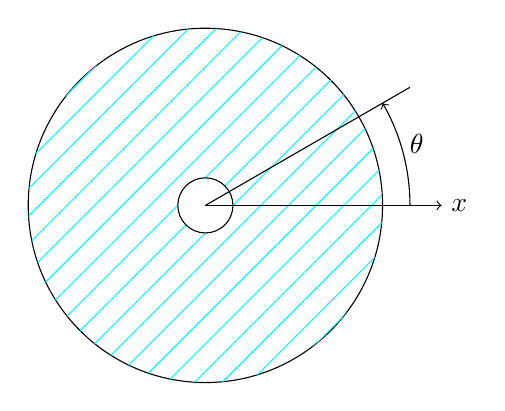
\begin{tikzpicture}
                % Draw the outer circle with hatching
                \draw (0,0) circle (2.25cm);
                \fill[pattern=north east lines dense, pattern color=cyan] (0,0) circle (2.25cm);
                % Draw the inner circle
                \draw[fill=white] (0,0) circle (0.35cm); % Fill with white to create the annular region
                % Draw the x and y axis
                \draw[->] (0,0) -- (3,0) node[right] {$x$};
                % Draw the angle theta
                \draw[->] ({3*cos(30)},0) arc (0:30:{3*cos(30)});
                \node at ({3.1*cos(30)}, {3*sin(15)}) {$\theta$};    
                % Draw a line showing the subtended angle
                \draw[-] (0,0) -- ({3*cos(30)}, {3*sin(30)});
            \end{tikzpicture}
            \caption{Voorbeeld van een tikZ afbeelding}
            \label{fig:sketch}
    \end{minipage}%
    \hspace{0.05\textwidth}
    \begin{minipage}{0.45\textwidth}
        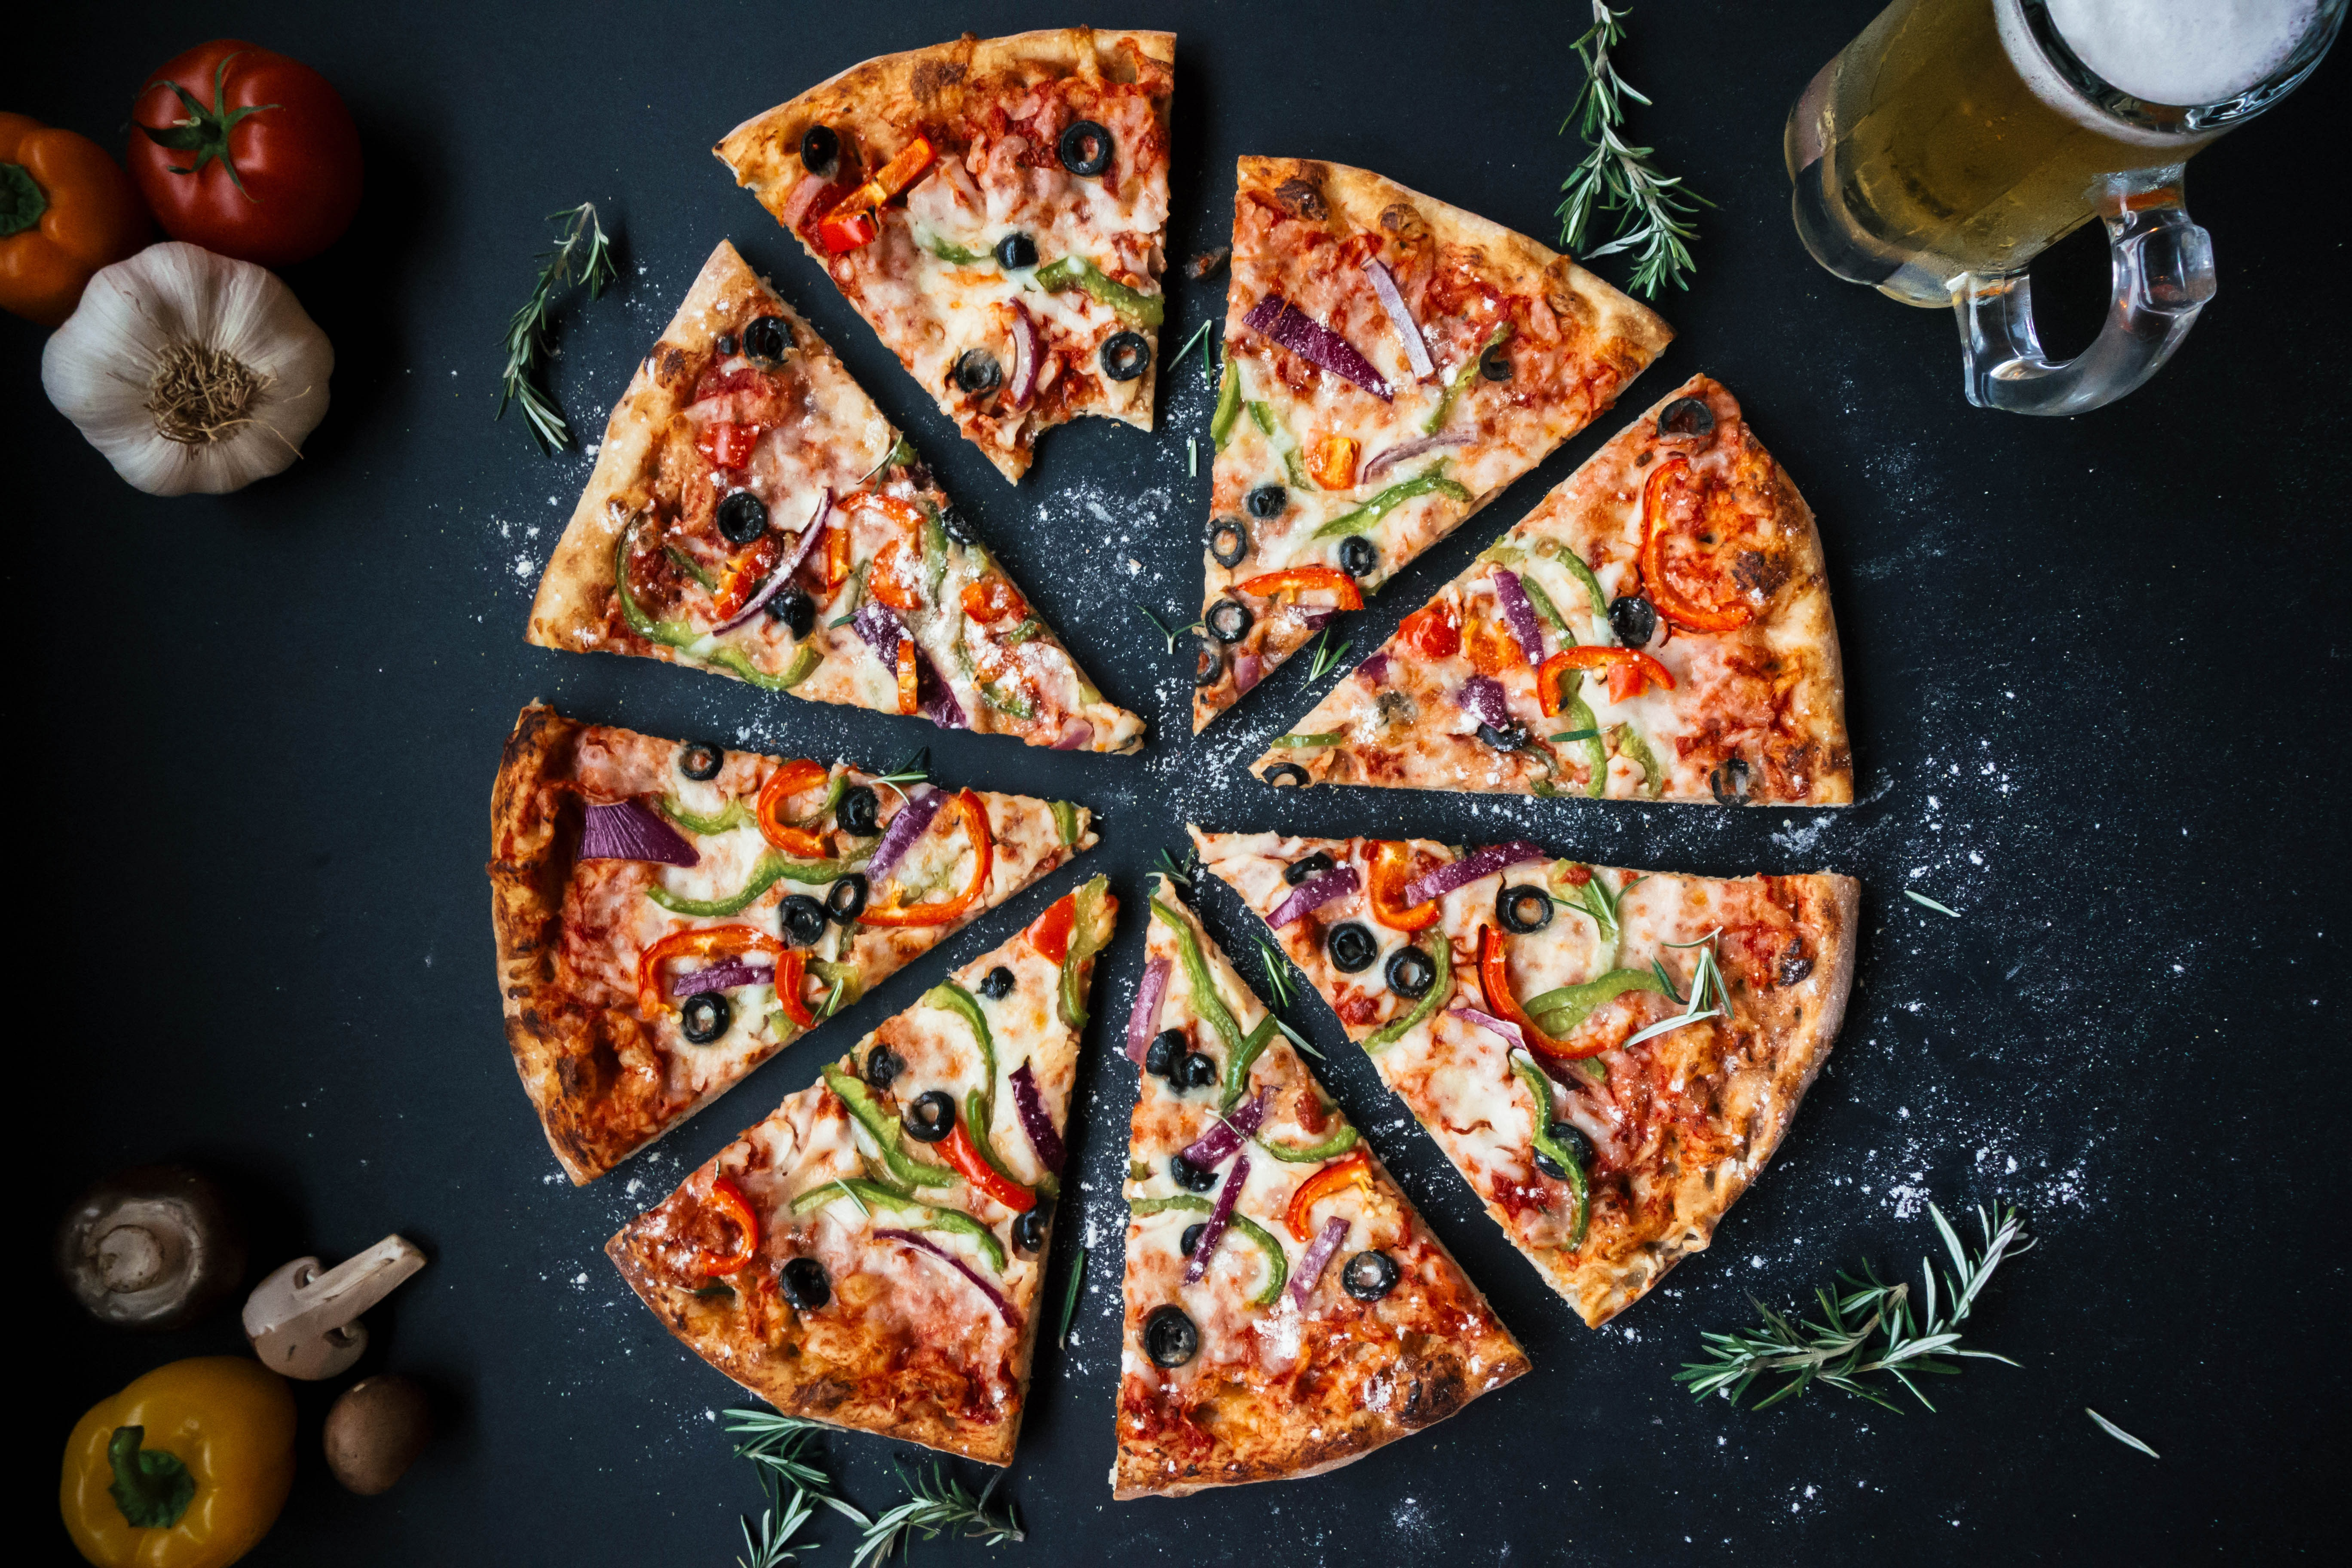
\includegraphics[width=\textwidth]{img/pizza.jpeg}
        \caption{Ik wist niet wat toevoegen dus hier is een pizza}
        \label{fig:pizza}
    \end{minipage}
    \caption{Merk op dat ik zowel de individuele figuren een onderschrift kan geven als beide tegelijk. Het enige verschil is de plaats van de caption en label.}
    \label{fig:minipage_example}
\end{figure}


\section{Tabellen}
% En een voorbeeld van een tabel
\begin{table}[H]
\centering
\caption{Plotting tool dependencies}
\label{tab:dependencies}
\begin{tabular}{l|l|l}
\rowcolor[HTML]{EFEFEF} 
Data & GUI & Built-in \\ \hline\hline
Plotly v5.11.0 & PyQt5 v5.15.4 & datetime \\ 
Numpy v1.24.0 & natsort v8.2.0 & json \\ 
Pandas v1.5.2 &  & csv \\ 
 &  & sys \\ 
 &  & os \\ 
\end{tabular}
\end{table}

Ook voor tabellen en figuren heeft Overleaf nuttige informatie\cite{OverleafFigures}, voor minipages kan je kijken op StackExchange\cite{StackExchangeMinipage}.

\section{Code snippets}
Hieronder heb ik de package \textit{listings} gebruikt die keywords bevat voor veel bekende talen zoals Python en C++.
Let echter op daar listings beschouwd worden als floating.

\begin{lstlisting}[language=C++]
class Particle {
public:
    // Constructor
    Particle(double mass, double charge) 
        : mass(mass), charge(charge) {}

    // Getters
    double getMass() const { return mass; }
    double getCharge() const { return charge; }

    // Setters
    void setMass(double m) { mass = m; }
    void setCharge(double c) { charge = c; }

private:
    double mass;
    double charge;
};
\end{lstlisting}
\begin{lstlisting}[language=Python,label=listing:python,caption=Python example with caption and label]    
import webbrowser

def open_youtube_video():
    url = "https://www.youtube.com/watch?v=dQw4w9WgXcQ"
    webbrowser.open(url)
open_youtube_video()
\end{lstlisting}

Dit bekom je dankzij de volgende structuur (hier letterlijk geplaatst dankzij de package \textit{verbatim}):
\begin{verbatim}
    \begin{lstlisting}[language=Python,label=listing:python,
    caption=Python example with caption and label]    
    import webbrowser
    
    def open_youtube_video():
        url = "https://www.youtube.com/watch?v=dQw4w9WgXcQ"
        webbrowser.open(url)
    open_youtube_video()
\end{lstlisting}
\end{verbatim}

\section{Referenties}
% Merk op dat elke zin op een aparte regel staat. Dit laat toe sneller problemen op te lossen daar LaTeX altijd een regelnummer geeft bij een error.
Je kan refereren naar labels in je tekst/figure/tabellen etc. door bijvoorbeeld \verb|\ref{fig:pikachu}| te gebruiken.
Zo verwijst \LaTeX ~automatisch naar het juiste nummer van de figuur: \ref{fig:pikachu}.
Beter is om de cleveref package en het commando \verb|\cref{tab:dependencies}| te gebruiken zodat LaTeX ook zelf refereert naar het type object.
Zo weet latex zelf dat ik refereer naar \cref{fig:pikachu} en \cref{tab:dependencies} of zelfs \cref{sec:intro}.
Je kan zelfs meerdere referenties samenvoegen met een comma zoals hier om te refereren naar \cref{fig:pizza,fig:minipage_example}.
Dit zal afhangen van de taalinstellingen in je preamble, gebruik hiervoor de juiste instellingen van de \textit{babel} package.
% Een lege regel of witregel geeft aan dat een nieuw paragraaf begonnen is

Het is ook mogelijk om LaTeX je bibliografie te laten beheren.
Gebruik daarvoor de \textit{csquotes} en \textit{biblatex}.
Je dient in de preamble ook te wijzen naar een \textit{references.bib} bestand met \verb|addbibresource| en \verb|\printbibliography| gebruiken waar je de lijst van referenties wilt toevoegen.
Zo kan ik enkele handige pagina's van Overleaf citeren \cite{Overleaf30min}.
Het document heb ik aangevuld met meerdere dergelijke referenties.

\printbibliography
\end{document}
